% (c) 2006 Ben Crowell, licensed under the Creative Commons
% Attribution-ShareAlike license,
% http://creativecommons.org/licenses/by-sa/1.0/
% and GFDL 1.2, http://www.gnu.org/copyleft/fdl.html .
%
\documentclass{lmseries}
% \let\ifpdf\relax % http://tex.stackexchange.com/questions/11414/package-ifpdf-error
% --------> this fails with TeX Live 2013, conflicts with xparse
%\selectlanguage{english}
\usepackage{lmlanguage}
%\includeonly{ch05/ch05}
\inputprotcode
\makeindex
\pdfmapfile{=fullembed.map} % created by the script create_fullembed_file
\begin{document}
\myeqnspacing % Do this early and often, since it gets reset by \normalsize
% 
% The following is all related to margin kerning.
% This is activated in dp.cls using the boolean wantmarginkerning.
% The constant 1 is to allow margin kerning, but to keep it from affecting
% line breaks.
\ifthenelse{\boolean{wantmarginkerning}}{
 \setprotcode\font
 {\it \setprotcode \font}
 {\bf \setprotcode \font}
 {\bf \it \setprotcode \font}
 \pdfprotrudechars=1
}{}
%========================= frontmatter =========================
\formatchtoc{\Large}{}{4mm}
\frontmatter
\yesiwantarabic
\renewcommand{\chapdir}{ch00}
\thispagestyle{empty}
\raisebox{0mm}[0mm][0mm]{%
\parbox{8.5in}{
\vspace*{236mm}\hspace{-38.5mm}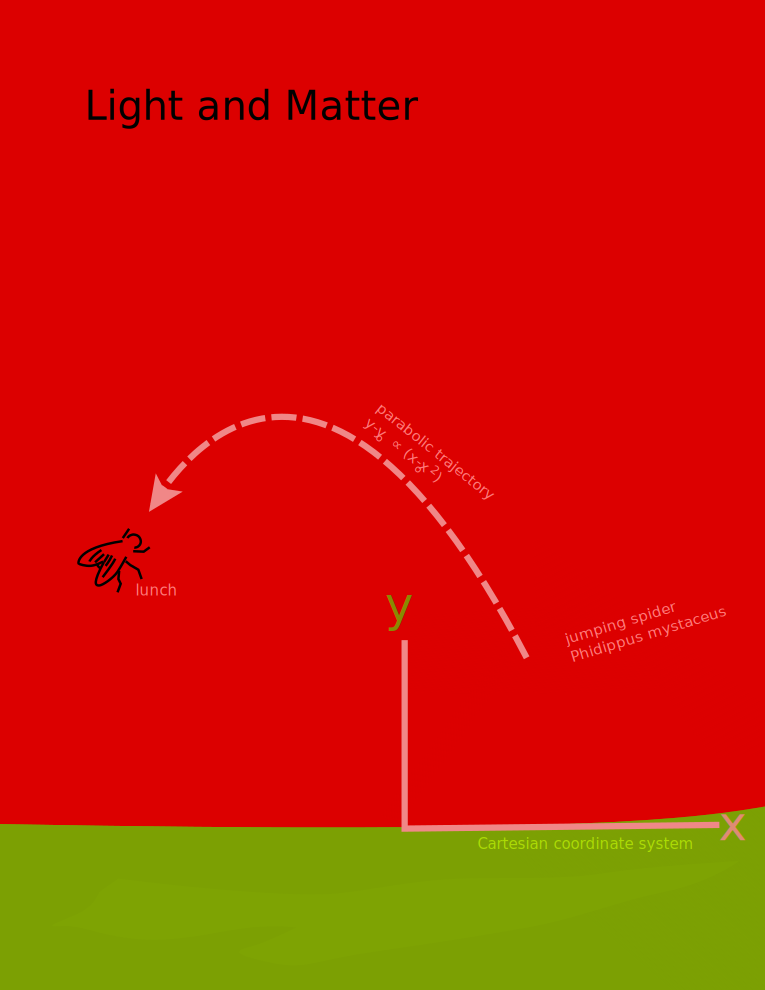
\includegraphics{\chapdir/figs/cover}\\
}
}%
\\

\pagebreak[4]

  \zerosizebox{-10mm}{140mm}{
    \noindent{}copyright 2006 Benjamin Crowell\vspace{10mm}
  }

  \zerosizebox{-10mm}{159mm}{
    rev. \today\vspace{10mm}
  }



  \zerosizebox{-10mm}{213mm}{
    \noindent{}\begin{minipage}{100mm}
    \noindent{}\begin{tabular}{p{9mm}p{95mm}}
    \zerosizebox{0mm}{14mm}{\anonymousinlinefig{cc-by-sa}} &
    This book is licensed under the 
Creative Commons
Attribution-ShareAlike license, version 3.0,
http://creativecommons.org/licenses/by-sa/3.0/,
    except for those photographs and
    drawings of which I am not the author, as listed in the photo credits.
    If you agree to the license, it grants you certain privileges that
    you would not otherwise have, such as the right to copy the book,
    or download the digital version free of charge from
    www.lightandmatter.com. At your option, you may also copy this book
    under the GNU Free Documentation License version 1.2, http://www.gnu.org/licenses/fdl.txt,
    with no invariant sections, no front-cover texts, and no back-cover texts.
    \end{tabular}
    \end{minipage}
}

\yesiwantarabic
\nomarginlayout
\onecolumn\pagebreak[4]
\noindent\huge\bfseries\sffamily{}\vspace{20mm}

\vspace{2mm}\hbox{}

\hspace{26mm}\hspace{5mm}\noindent{}Brief Contents

\vspace{0mm}\hbox{}

\hspace{20mm}\noindent\mynormaltype\Large\sffamily{}\begin{tabular}{rl}
\brieftocentrywithlink{ch:intro}{Introduction and review} \\
\brieftocentrywithlink{ch:scaling}{Scaling and estimation} \\
\brieftocentrywithlink{ch:motion}{Velocity and relative motion} \\
\brieftocentrywithlink{ch:acceleration}{Acceleration and free fall} \\
\brieftocentrywithlink{ch:newton}{Force and motion} \\
\brieftocentrywithlink{ch:forces}{Analysis of forces} \\
\brieftocentrywithlink{ch:three-d}{Newton's laws in three dimensions} \\
\brieftocentrywithlink{ch:vectors}{Vectors} \\
\brieftocentrywithlink{ch:vectors-and-motion}{Vectors and motion} \\
\brieftocentrywithlink{ch:circular-motion}{Circular motion} \\
\brieftocentrywithlink{ch:gravity}{Gravity} \\
\brieftocentrywithlink{ch:energy}{Conservation of energy} \\
\brieftocentrywithlink{ch:energy-zoo}{Simplifying the energy zoo} \\
\brieftocentrywithlink{ch:work}{Work: the transfer of mechanical energy} \\
\brieftocentrywithlink{ch:momentum}{Conservation of momentum} \\
\brieftocentrywithlink{ch:angular-momentum}{Conservation of angular momentum} \\
\brieftocentrywithlink{ch:thermo}{Thermodynamics} \\
\brieftocentrywithlink{ch:vibrations}{Vibrations} \\
\brieftocentrywithlink{ch:resonance}{Resonance} \\
\brieftocentrywithlink{ch:free-waves}{Free waves} \\
\brieftocentrywithlink{ch:bounded-waves}{Bounded waves} \\
\brieftocentrywithlink{ch:circuits}{Electricity and circuits} \\
\brieftocentrywithlink{ch:fields}{The nonmechanical universe} \\
\brieftocentrywithlink{ch:relativity}{Relativity and magnetism} \\
\brieftocentrywithlink{ch:em}{Electromagnetism} \\
\brieftocentrywithlink{ch:lrc}{Capacitance and inductance} \\
\brieftocentrywithlink{ch:atom}{The atom and E=mc$^2$} \\
\brieftocentrywithlink{ch:genrel}{General relativity} \\
\brieftocentrywithlink{ch:ray-model}{The ray model of light} \\
\brieftocentrywithlink{ch:images-1}{Images by reflection} \\
\brieftocentrywithlink{ch:images-2}{Images, quantitatively} \\
\brieftocentrywithlink{ch:refraction}{Refraction} \\
\brieftocentrywithlink{ch:wave-optics}{Wave optics} \\
\brieftocentrywithlink{ch:randomness}{Rules of randomness} \\
\brieftocentrywithlink{ch:light-as-a-particle}{Light as a particle} \\
\brieftocentrywithlink{ch:matter-as-a-wave}{Matter as a wave} \\
\brieftocentrywithlink{ch:qm-atom}{The atom} \\

\end{tabular}

\vspace{12mm}

\mynormaltype\sffamily{}
\noindent 
For a semester-length course, all seven chapters can be covered.
For a shorter course, the book is designed so that chapters 1, 2, and 5 are the only
ones that are required for continuity; any of the others can be included or
omitted at the instructor's discretion, with the only constraint being that
chapter 6 requires chapter 4.

\vspace{12mm}\hbox{}


\vfill
\mynormaltype

\pagebreak[4]

\vspace{0mm}
\begin{center}
\noindent\huge\bfseries\sffamily{}Contents\mynormaltype
\end{center}
\vspace{0mm}
\begin{multicols}{2}
  \tableofcontents
  \setcounter{unbalance}{0}
\end{multicols}
\normallayout\onecolumn

%========================= main matter =========================
\mainmatter
%-- I want the whole book numbered sequentially, arabic:
  \pagenumbering{arabic} 
  \addtocounter{page}{6} 
\parafmt
\myeqnspacing % Do this early and often, since it gets reset by \normalsize
%========================= chapters =========================
	\renewcommand{\chapdir}{ch01}\include{ch01/ch01temp}\write18{../mv_silent all.pos ch01.pos}% 
\wugga
	\renewcommand{\chapdir}{ch02}\include{ch02/ch02temp}\write18{../mv_silent all.pos ch02.pos}% 
	\renewcommand{\chapdir}{ch03}\include{ch03/ch03temp}\write18{../mv_silent all.pos ch03.pos}% 
	\renewcommand{\chapdir}{ch04}\include{ch04/ch04temp}\write18{../mv_silent all.pos ch04.pos}% 
	\renewcommand{\chapdir}{ch05}\include{ch05/ch05temp}\write18{../mv_silent all.pos ch05.pos}% 
	\renewcommand{\chapdir}{ch06}\include{ch06/ch06temp}\write18{../mv_silent all.pos ch06.pos}% 
	\renewcommand{\chapdir}{ch07}\include{ch07/ch07temp}\write18{../mv_silent all.pos ch07.pos}% 
	\formatchtoc{\large}{\quad\contentspage}{4mm} % This has to go before the last chapter.
	\renewcommand{\chapdir}{ch08}\include{ch08/ch08temp}\write18{../mv_silent all.pos ch08.pos}% 
%========================= backmatter =========================
\getreadyforbackmatter
\backmatter
\renewcommand{\chapdir}{ch99}
%========================= appendices =========================
\formatchtoc{\large}{\quad\contentspage}{0mm} % This has to go before first appendix.
\renewcommand{\chaptermark}[1]%
    {\markboth{\textsf{\thechapter\hspace{\myfooterspace}#1}}{}}
% exercises
%        \newpage\include{ch99/exercises}
% photo credits
	\newpage
\refstepcounter{appendixctr}\label{photocreditsappendix}%
\appendix\chapter{Appendix \ref{photocreditsappendix}: Photo Credits}
Except as specifically noted below or in a parenthetical credit in the
caption of a figure, all the illustrations in this book are by
under my own copyright, and are copyleft licensed under the same license
as the rest of the book. 

In some cases it's clear from the date that the
figure is public domain, but I don't know the name of the artist or photographer; I would
be grateful to anyone who could help me to give proper credit.
I have assumed that images
that come from U.S. government web pages are copyright-free, since products
of federal agencies fall into the public domain.
When ``PSSC Physics'' is given as a credit, it indicates that the figure
is from the second edition of the textbook entitled Physics, by the
Physical Science Study Committee; these are used according to a blanket
permission given in the later PSSC College Physics edition, which states
on the copyright page that ``The materials taken from the original and second
editions and the Advanced Topics of PSSC PHYSICS included in this text
will be available to all publishers for use in English after December 31, 1970,
and in translations after December 31, 1975.'' 

In a few cases, I have made use of images under the fair use doctrine. However,
I am not a lawyer, and the laws on fair use are vague, so you should not assume
that it's legal for you to use these images. In particular, fair use law may
give you less leeway than it gives me, because I'm using the images for
educational purposes, and giving the book away for free. Likewise, if the
photo credit says ``courtesy of ...,'' that means the copyright owner gave
me permission to use it, but that doesn't mean you have permission to use it.

\begin{sloppypar}
\noindent
\textbf{Cover}
\barecred{Wave}{Roger McLassus, GFDL 1.2}
\barecred{Hand and photomontage}{B. Crowell}
\end{sloppypar}

\begin{sloppypar}
\noindent
\textbf{Table of Contents}
\barecred{Skateboarder}{Courtesy of J.D. Rogge, www.sonic.net/$\sim$shawn}
\barecred{Figure skater}{Wikimedia Commonus user Rosiemairieanne, GFDL 2}
\barecred{Sunspot}{Royal Swedish Academy of Sciences. The astronomers' web page at
    http://www.solarphysics.kva.se/NatureNov2002/press\_images\_eng.html states ``All images are free for publication.''}
\barecred{X-Ray}{1896 image produced by Roentgen}
\barecred{Surfing}{Stan Shebs, GFDL licensed (Wikimedia Commons)}
\end{sloppypar}

\begin{sloppypar}
\noindent
\cred{startrails}{Star trails}{GFDL licensed, Wikipedia user Manfreeed}
\cred{noether}{Emmy Noether}{Based on Noether's apparent age, the portrait
                     must have been taken around 1900 or 1910, so it is in the public domain}
\cred{c-s-wu-with-beamline}{C.S.~Wu}{Smithsonian Institution, believed to be public domain}% http://en.wikipedia.org/wiki/File:Chien-shiung_Wu_%281912-1997%29.jpg
\cred{swan-lake-symmetry}{Swan Lake}{Peter Gerstbach, GFDL 1.2}
\cred{lavoisier}{Portrait of Monsieur Lavoisier and His Wife}{Jacques-Louis David, 1788}
\cred{bodymass}{Astronaut}{NASA}
\cred{hockey-puck}{Hockey puck}{photo from Wikimedia Commons, user Robludwig, GFDL/CC-BY-SA}
\cred{joule}{Portrait of James Joule}{contemporary}
\cred{aristotle}{Aristotle}{Francesco Hayez, 1811}
\cred{jets-in-formation-over-ny}{Jets over New York}{U.S. Air Force, Tech. Sgt. Sean Mateo White, public domain work of the U.S. Government}%http://en.wikipedia.org/wiki/Image:F-16_Fighting_Falcons_above_New_York_City%282%29.jpg
\cred{galileo-trial}{Galileo's trial}{Cristiano Banti (1857)}
\cred{rocket-sled}{Rocket sled}{U.S. Air Force, public domain work of the U.S. Government}
\cred{foucault}{Foucault and pendulum}{contemporary, ca. 1851}
\cred{pool-skater}{Skateboarder}{Courtesy of J.D. Rogge, www.sonic.net/$\sim$shawn}
\cred{welding}{Welding}{William M. Plate, Jr., public-domain product of the U.S. Airforce, Wikimedia Commons}
\cred{irbike}{Infrared photographs}{Courtesy of M. Vollmer and K.P. M\"{o}llmann, Univ. Appl. Sciences,
                        Brandenburg, Germany, www.fh-brandenburg.de/$\sim$piweb/projekte/thermo\_galerie\_eng.html}
\cred{newton}{Newton}{Godfrey Kneller, 1702}
\cred{eclipse}{Eclipse}{1919, public domain}
\cred{newspaper-eclipse}{Newspaper headline}{1919, public domain}
\cred{hw-colliding-balls}{Colliding balls}{PSSC Physics}
\cred{tycho-brahe}{Brahe}{public domain}
\cred{baseball-pitch}{Basebal pitch}{Wikipedia user Rick Dikeman, GFDL 1.2}%http://en.wikipedia.org/wiki/Image:Baseball_pitching_motion_2004.jpg
\cred{hw-posnegwork-bull}{Bull}{Photo by Wikimedia Commons user Bart Hiddink, CC-BY} % https://upload.wikimedia.org/wikipedia/commons/f/fd/Angry_Bull_in_Pasture.jpg
\docred{\pageref{ch:angular-momentum}}{Tornado}{NOAA Photo Library, NOAA Central Library; OAR/ERL/National Severe Storms Laboratory (NSSL); public-domain product of the U.S. government}
\cred{longjump}{Longjump}{Thomas Eakins, public domain}
\cred{conical-pendulum}{Pendulum}{PSSC Physics}
\cred{tetherball}{Tetherball}{Line art by the author, based on a photo by The Chewonki Foundation (Flickr), CC-BY-SA 2.0 licensed}
\cred{rhic}{Colliding nuclei}{courtesy of RHIC}
\cred{machine-gun-ftl}{Machine gunner's body}{Redrawn from a public-domain photo by Cpl.~Sheila Brooks}% http://commons.wikimedia.org/wiki/File:V-22_M240_machine_gun.jpg
\cred{machine-gun-ftl}{Machine gunner's head}{Redrawn from a sketch by Wenceslas Hollar, 17th century}% http://commons.wikimedia.org/wiki/File:Wenceslas_Hollar_-_Woman%27s_head_seen_from_behind.jpg
\docred{\pageref{lightning-photo-page}}{Lightning}{C. Clark/NOAA photo library, public domain}
\cred{ampere}{Amp\`{e}re}{Millikan and Gale, 1920}
\cred{volta}{Volta}{Millikan and Gale, 1920}
\cred{ohm}{Ohm}{Millikan and Gale, 1920}
\cred{sunspot}{Sunspot}{Royal Swedish Academy of Sciences. The astronomers' web page at
    http://www.solarphysics.kva.se/NatureNov2002/press\_images\_eng.html states ``All images are free for publication.''}
\cred{faraday}{Faraday banknote}{fair use}
\cred{young-maxwell}{Maxwell}{19th century photograph}
\docred{\pageref{ch:ray-model}}{Rays of sunlight}{Wikipedia user PiccoloNamek, GFDL 1.2}
\cred{io}{Jupiter and Io}{NASA/JPL/University of Arizona}
\cred{computer-ray-tracing}{Ray-traced image}{Gilles Tran, Wikimedia Commons, public domain}
\cred{angular-size}{Flower}{Based on a photo by Wikimedia Commons user Fir0002, GFDL 1.2}
\cred{newtonian-telescope-eye}{Moon}{Wikimedia commons image}
\docred{\pageref{ch:waves}}{Painting of waves}{Katsushika Hokusai (1760-1849), public domain}
\cred{john-hancock-tower}{John Hancock Tower}{Wikipedia user Sfoskett, GFDL 1.2}
\cred{coil-spring-superposition}{Superposition of pulses}{Photo from PSSC Physics}
\cred{ribbon-on-spring}{Marker on spring as pulse passes by}{PSSC Physics}
\cred{surfing-hand-drag}{Surfing (hand drag)}{Stan Shebs, GFDL licensed (Wikimedia Commons)}
\cred{breaking-wave}{Breaking wave}{Ole Kils, olekils at web.de, GFDL licensed (Wikipedia)}
\cred{circular-and-linear-wavelengths}{Wavelengths of circular and linear waves}{PSSC Physics}
\cred{ultrasound}{Fetus}{Image of the author's daughter}
\cred{wavelength-change}{Changing wavelength}{PSSC Physics}
\end{sloppypar}

% hw hints, answers, solutions	
	\onecolumn\refstepcounter{appendixctr}\label{hwansappendix}%
\appendix\chapter{Appendix \ref{hwansappendix}: Hints and Solutions}
	
%==================================================================
%==================================================================
%========================= Self-Checks ============================
%==================================================================
%==================================================================




\noindent\formatlikesection{Answers to Self-Checks}

%----------------------------------------------------------------------------------------

\noindent\formatlikesubsection{Answers to Self-Checks for Chapter \ref{ch:energy}}\\
\scanshdr{conservation} A conservation law in physics says that the total
amount always remains the same. You can't get rid of it even if you want to.

\scanshdr{bacteria-queue}
Exponents have to do with multiplication, not addition. The
first line should be 100 times longer than the second,
not just twice as long.

\scanshdr{mars-and-venus}
Doubling $d$ makes $d^2$ four times bigger, so the gravitational field experienced
by Mars is four times weaker.

%----------------------------------------------------------------------------------------

\noindent\formatlikesubsection{Answers to Self-Checks for Chapter \ref{ch:momentum}}\\
\scanshdr{moonviolatestranslation} No, it doesn't violate symmetry. Space-translation symmetry
only says that space itself has the same properties everywhere. It doesn't say that all regions
of space have the same stuff in them. The experiment on the earth comes out a certain way because
that region of space has a planet in it. The experiment on the moon comes out different because
that region of space has the moon in it. of the apparatus, which you forgot to take with you.

\scanshdr{markcm} The camera is moving at half the speed at which the light ball is initially
moving. After the collision, it keeps on moving at the same speed --- your five x's all line
on a straight line. Since the camera moves in a straight line with constant speed, it is
showing an inertial frame of reference.

\scanshdr{thirdframepcons} The table looks like this:

\velocitytable{$-1$}{0}{$+1$}{0}{$-1$}{$-1$}{../../../cp/ch02/figs/darkball}{../../../cp/ch02/figs/lightball}

\noindent Observers in all three frames agree on the changes in velocity, even though they disagree
on the velocities themselves.

\scanshdr{heavierball} The motion would be the same. The force on the ball would be 20 newtons,
so with each second it would gain 20 units of momentum. But 20 units of momentum for a 2-kilogram
ball is still just 10 m/s of velocity.

%----------------------------------------------------------------------------------------

\noindent\formatlikesubsection{Answers to Self-Checks for Chapter \ref{ch:angular-momentum}}\\
\scanshdr{importance-of-torque-equations}
The definition of torque is important, and so is the equation $F=\pm Fr$. The two equations
in between are just steps in a derivation of  $F=\pm Fr$.

%----------------------------------------------------------------------------------------

\noindent\formatlikesubsection{Answers to Self-Checks for Chapter \ref{ch:relativity}}\\
\scanshdr{unequalcollisioncons} The total momentum is zero before the collision. After the
collision, the two momenta have reversed their directions, but they still cancel.
Neither object has changed its kinetic energy, so the total energy before and after the collision
is also the same.

%----------------------------------------------------------------------------------------

\noindent\formatlikesubsection{Answers to Self-Checks for Chapter \ref{ch:electricity}}\\
\scanshdr{typesofcharge} Either type can be involved in either an attraction or a
repulsion. A positive charge could be involved in either an attraction (with a negative
charge) or a repulsion (with another positive), and a negative could participate
in either an attraction (with a positive) or a repulsion (with a negative).

\scanshdr{inductionneg} It wouldn't make any difference. The roles of the positive and
negative charges in the paper would be reversed, but there would still be a net attraction.

%----------------------------------------------------------------------------------------

\noindent\formatlikesubsection{Answers to Self-Checks for Chapter \ref{ch:fields}}\\
\scanshdr{alternator}
An induced electric field can only be created by a \emph{changing} magnetic
field. Nothing is changing if your car is just sitting there. A point on the
coil won't experience a changing magnetic field unless the coil is already
spinning, i.e., the engine has already turned over.

%----------------------------------------------------------------------------------------

\noindent\formatlikesubsection{Answers to Self-Checks for Chapter \ref{ch:ray-model}}\\
\scanshdr{two-reflections-from-same-point}
Only 1 is correct. If you draw the normal that bisects the solid ray, it
also bisects the dashed ray.

\scanshdr{candlefivetimes}{He's five times farther away than she is, so the light he sees
is 1/25 the brightness.}

\scanshdr{move-object-laterally} You should have found from your ray diagram
that an image is still formed, and it has simply moved down the same distance
as the real face. However, this new image would only be visible from high up,
and the person can no longer see his own image. 

\scanshdr{real-do-and-di}
Increasing the distance from the face to the mirror has decreased the distance
from the image to the mirror. This is the opposite of what happened with the virtual
image.

%----------------------------------------------------------------------------------------

\noindent\formatlikesubsection{Answers to Self-Checks for Chapter \ref{ch:waves}}\\
\scanshdr{ribbon-on-spring}
The leading edge is moving up, the trailing edge is moving down, and the top of the
hump is motionless for one instant.

%==================================================================
%==================================================================
%========================= Solutions ==============================
%==================================================================
%==================================================================

\hwanssection{Solutions to Selected Homework Problems}

\beginsolutions{energy}

\hwsolnhdr{mg-to-kg}

\begin{equation*}
  134\ \zu{mg} \times \frac{10^{-3}\ \gunit}{1\ \zu{mg}} \times \frac{10^{-3}\ \kgunit}{1\ \zu{g}} = 1.34\times10^{-4}\ \kgunit
\end{equation*}

\beginsolutions{angular-momentum}
\hwsolnhdr{pliers}
The pliers are not moving, so their angular momentum
remains constant at zero, and the total torque on them must
be zero. Not only that, but each half of the pliers must
have zero total torque on it. This tells us that the
magnitude of the torque at one end must be the same as that
at the other end. The distance from the axis to the nut is
about 2.5 cm, and the distance from the axis to the centers
of the palm and fingers are about 8 cm. The angles are close
enough to $90\degunit$ that we can pretend they're 90 degrees,
considering the rough nature of the other assumptions and
measurements. The result is $(300\ \nunit)(2.5\ \zu{cm})=(F)(8\ \zu{cm})$,
 or $F=90$ N.

%========================= index =========================
\printindex
\end{document}
